The results of the four fits for the irregular dust grains are presented in Table \ref{tab: dust_model_fits_irregular} and Figure \ref{fig: irregular_fits}. The lowest $\chi_\mathcal{P}^2$ occurs for the no \bsix fit case, however, the all-wavelengths case gives a very similar result. Both cases have a best-fit grain size of 212 \micronNS. 



\begin{table}[h!]
\centering
\caption{Same as Table \ref{tab: dust_model_fits_spherical} but for irregular grains. Note that for the irregular grains, porosity is not varied.}
\begin{tabular}{lccc}
\toprule
\textbf{Fit Case} &  \textbf{Scale Factor (SF)} & $\boldsymbol{\chi_\mathcal{P}^2}$ & \textbf{$\boldsymbol{\amaxEQ}$ ($\boldsymbol{\mu}$m)} \\
\midrule

All wavelengths         & 1.77 & 4.58 & 212 \\
No \bfive               & 1.81 & 6.16 & 214 \\
No \bsix                & \textbf{1.79} & \textbf{4.39} & \textbf{212} \\
Just \bfour and \bseven & 1.83 & 8.41 & 215 \\

\bottomrule
\end{tabular}
\label{tab: dust_model_fits_irregular}
\end{table}






\begin{figure*}[h]
  \centering
  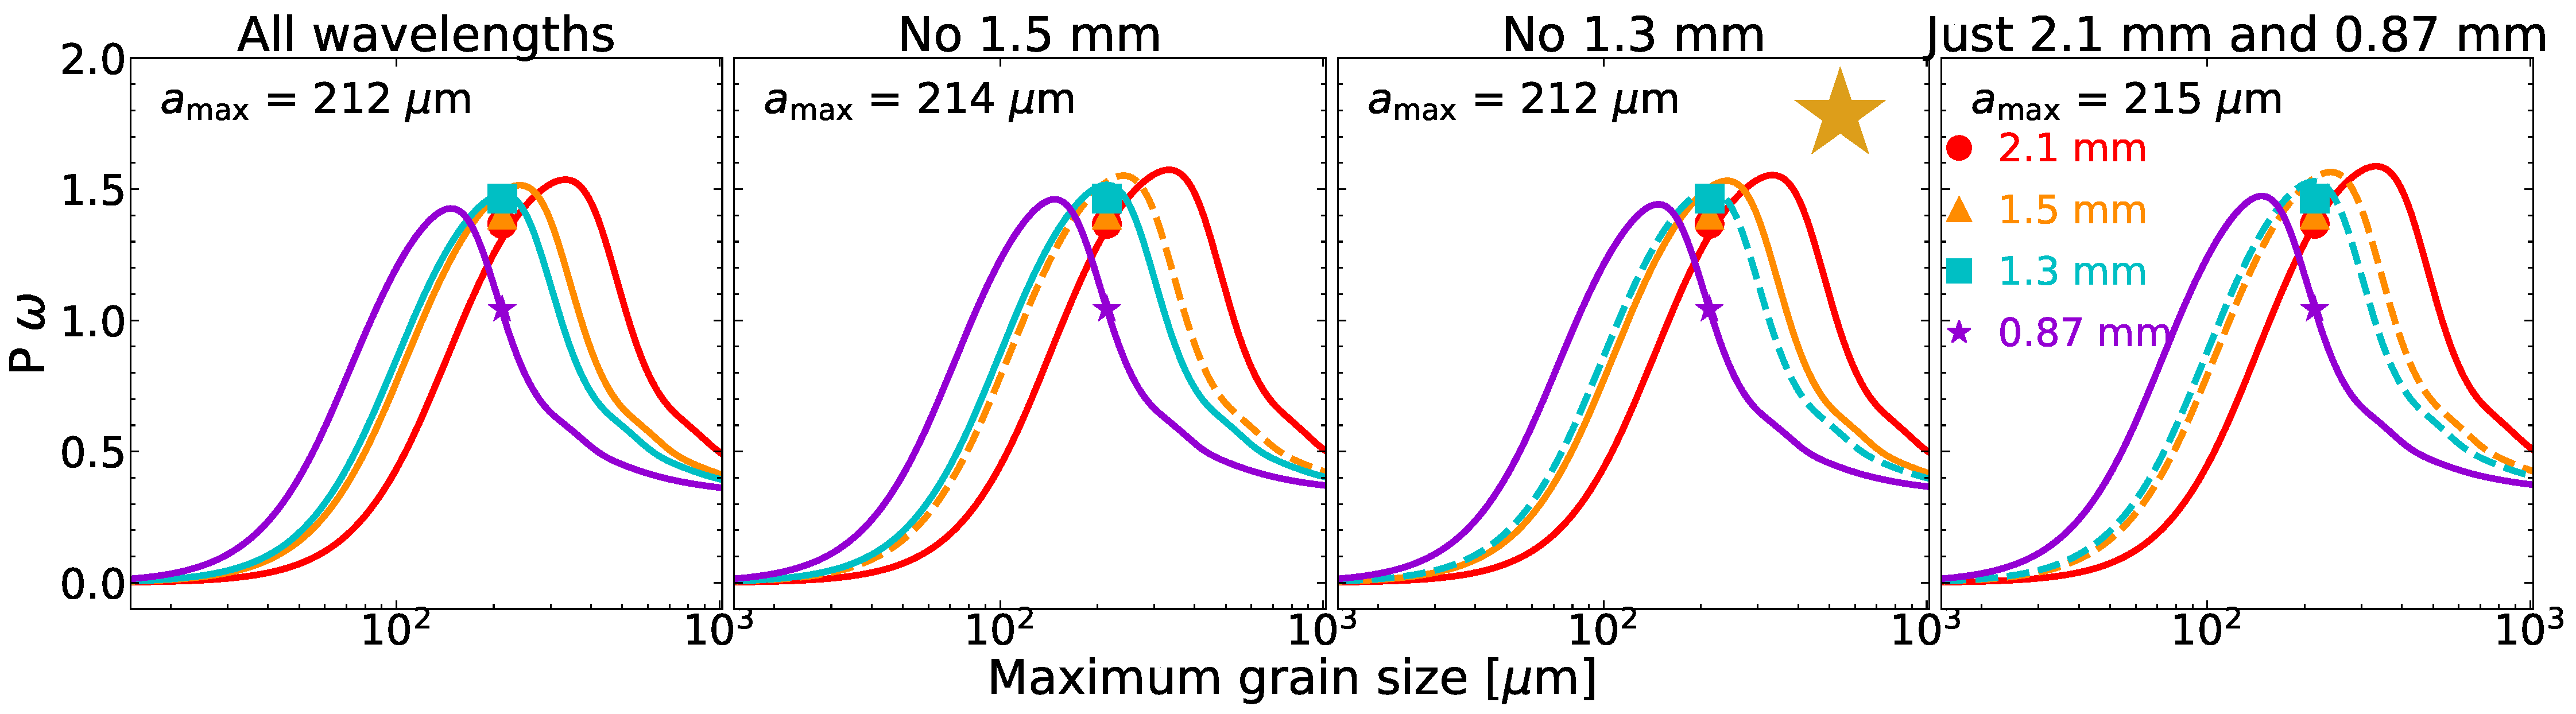
\includegraphics[width=1.1\textwidth]{../IMAGES/WRITEUP/glitterin/DustModelPlot_GlitterinGrid.pdf}
  \caption{Same as Figure \ref{fig: Spherical_BEST} but for irregular dust grains. Porosity is not varied, but each fit is represented in the grid. Corresponding results can be found in Table \ref{tab: dust_model_fits_irregular}. \question{Do I need the titles, or are the dashed lines clear enough?} \note{Legend overlaps with curves a bit; can make text smaller.}}
  \label{fig: irregular_fits}
\end{figure*}



% \begin{figure*}[h]
%   \centering
%   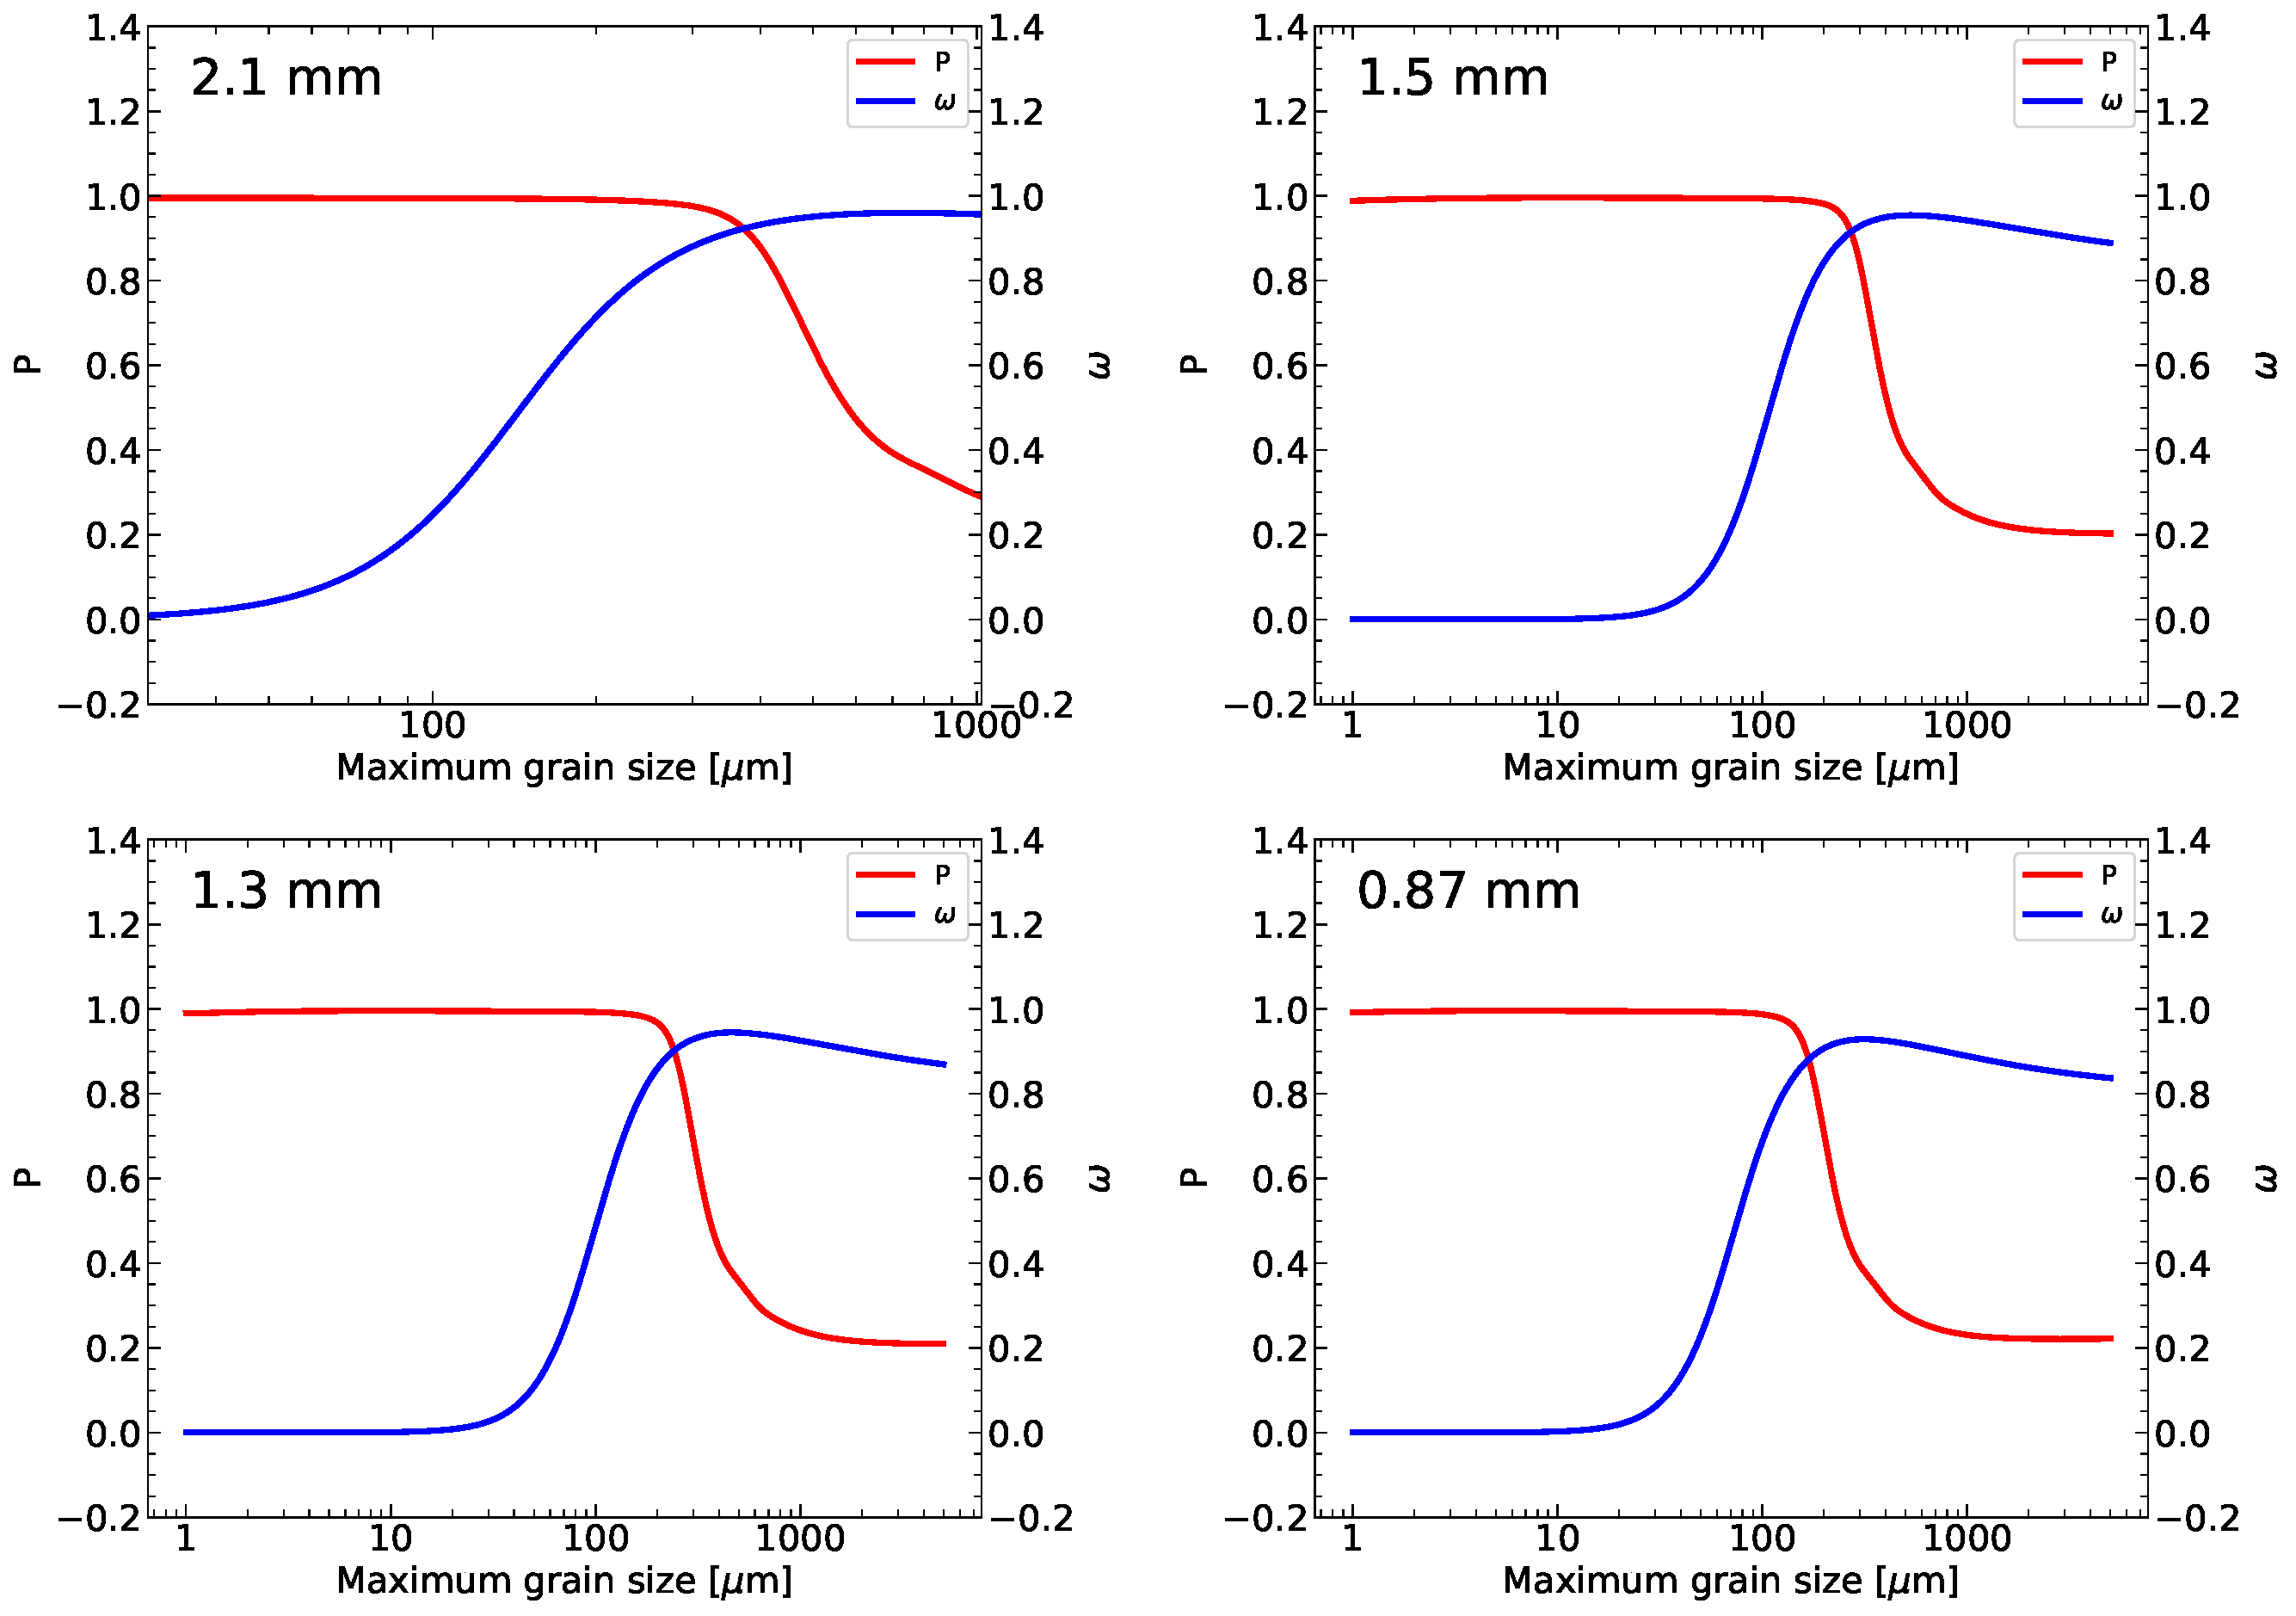
\includegraphics[width=1.1\textwidth]{WRITEUP_AND_IMAGES/IMAGES/WRITEUP/glitterin/P_vs_w_vs_grainsize_grid.pdf}
%   \caption{\add{caption} \question{Make this one row to take up less space, or will that be too small?}}
%   \label{fig: Kataoka2015Figure3Recreation_glitterin}
% \end{figure*}